\documentclass{article}
\usepackage{geometry}
 \geometry{
 a4paper,
 bottom=10mm,
 right=20mm,
 left=20mm,
 top=10mm,
 }

\usepackage[dvipsnames]{xcolor}
\usepackage{tikz}
\usetikzlibrary{calc}
\usepackage{graphics}
\usepackage{amsmath}
\usepackage{amssymb}
\tikzset{>=stealth}

\usepackage{hyperref}
\usepackage{setspace}
\onehalfspacing

\begin{document}

\noindent In the following we derive analytical expressions for $y_i$ and $y_f$. 
Those values are needed to specify entrance and endpoint of the rays at the outer circle (API by \texttt{RadonKA.jl}\footnote{\url{www.github.com/roflmaostc/RadonKA.jl}}).
Given the circular shaped vial, the angle under which a ray hits the vial is $\alpha = \arcsin(y / R_o)$. Consequently, because of refraction we obtain $\beta=\arcsin(\sin(\alpha) / n_\text{vial})$.
The orange segment $x$ is more inconvenient to derive but the law of cosines of triangles provides us with 
\begin{equation}
    R_i^2 = x^2 + R_o^2 - 2 \cdot x \cdot R_o \cos{\beta}.
\end{equation}
Solving the quadratic equation, the meaningful solution is
\begin{equation}
    x = R_o \cdot \cos{\beta} -  \sqrt{R_o^2 \cdot (\cos(\beta)^2 - 1) + R_i^2}.
\end{equation}
Again, applying law of cosine we can obtain an expression for
\begin{equation}
    \varepsilon = \arccos\left(\frac{x^2 + R_i^2 - R_o^2}{2 R_i x}\right) - \frac{\pi}{2}.
\end{equation}
Further, $\beta'=\mathrm{sign}(y) \cdot (\frac{\pi}{2}- \varepsilon)$ and because of refraction $\gamma=\arcsin(\frac{n_\text{vial} \cdot \sin(\beta')}{n_\text{resin}})$. 
The total ray deflection angles are given by $\delta_1=\alpha - \beta$ and $\delta_2=\beta-\gamma$ resulting in $\delta_\text{ges} = \delta_1 + \delta_2$. 

% $\Delta y$ indicates the height distance the ray propagates because of refraction on the vial interface and is given by $\Delta y = \sin(\delta_1) \cdot x$. 
% The horizontal distance from beginning of the vial until intersection with the vial is given by $\Delta x = R_o - \sqrt{R_o^2-y^2}$.
% Similarly, the horizontal distance from entrance of the vial until intersection with the resin is given by $\Delta x_2 = \sqrt{x^2-\Delta y^2}$.
% Finally, we arrive at $y_f$ which is the absolute vertical position of the ray at the horizontal ending of the vial.
\noindent
To calculate the height $y_i$ which describes the virtual height while entering the outer circle, we first need the distance $y' = R_i \cdot \sin(\gamma)$.
Using the Pythagorean theorem we can derive
\begin{equation}
    p = \sqrt{R_o^2-y'^2}.
\end{equation}
Then, the angle $\eta$ is given by
\begin{equation}
    \eta =- \left(\arcsin\left(\frac{y'}{R_0}\right) - \text{sign}(y) \cdot \left(\frac{\pi}{2}-\delta_{\text{ges}}\right)\right)
\end{equation}
Then, the height of the ray at exiting the outer circle, is given by 
\begin{equation}
    y_f = R_o \cdot \sin(\eta). 
\end{equation}
Because of the isosceles triangle, the height of the virtual ray entering the outer circle is given by
\begin{equation}
    y_i =  2\cdot p \cdot \sin(\delta_\text{ges}) + y_f 
\end{equation}

\begin{figure}[h] 
\centering
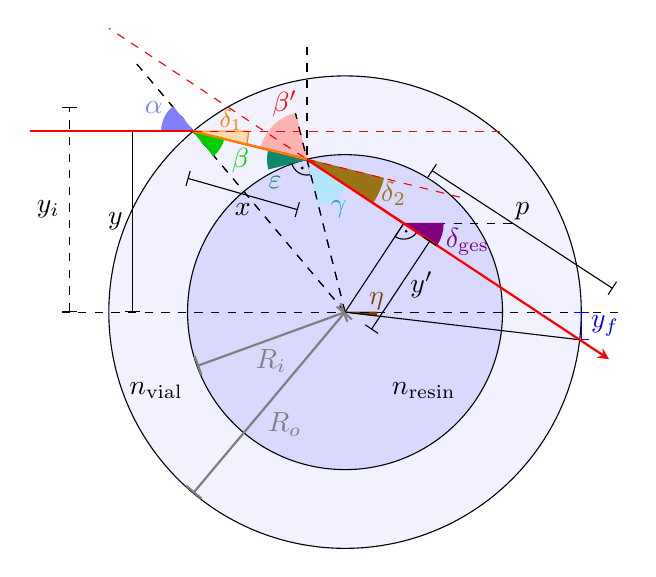
\begin{tikzpicture}
    \def\R{3};
    \def\Ri{2};
    \def\alph{50};
    \def\n{1.3};
    \def\ntwo{1.7};
    \draw[fill=blue!5!white] (0,0) circle(\R);
    \draw[fill=blue!15!white] (0,0) circle(\Ri);
    
    \pgfmathsetmacro\y{{{\R * sin(\alph)}}};
    \pgfmathsetmacro\x{{{\R * cos(\alph)}}};
    \pgfmathsetmacro\bet{{{asin(sin(\alph) / \n)}}};
    %\pgfmathsetmacro\xdist{{{1.4884}}};
    \pgfmathsetmacro\xdist{{{\R * cos(\bet) - sqrt(-\R^2/2 + \Ri^2 + 0.5 * \R^2 * cos(2 * \bet))}}};

    \pgfmathsetmacro\epsilo{{{acos((-\R^2 + \xdist^2 + \Ri^2) / 2 / \Ri / \xdist) - 90}}};
    \pgfmathsetmacro\bettwo{{{90 - \epsilo}}};
    \pgfmathsetmacro\gamm{{{asin(\n * sin(\bettwo) / \ntwo)}}};
    
    \pgfmathsetmacro\delt{{{\alph-\bet}}}; 
    \pgfmathsetmacro\delttwo{{{\bettwo - \gamm}}}; 
    \pgfmathsetmacro\deltges{{{\alph-\bet + \bettwo - \gamm}}}; 
    \pgfmathsetmacro\gimmel{{{180-\gamm-\deltges}}}
    \pgfmathsetmacro\deltax{{{\R - sqrt(\R^2-\y^2)}}}
    \pgfmathsetmacro\deltah{{{sin(\delt) * \xdist}}}
    \pgfmathsetmacro\deltaxtwo{{{sqrt(\xdist^2-\deltah^2)}}}
    \pgfmathsetmacro\ythree{{{\y - \deltah - tan(\delt + \delttwo) * (2 * \R - \deltax - \deltaxtwo)}}}
    \pgfmathsetmacro\yi{{{\ythree+tan(\deltges)*2*\R}}}

    \pgfmathsetmacro\yy{\y/\n};
    \pgfmathsetmacro\yyy{{{sin(\gamm) * \Ri}}}
    
    \pgfmathsetmacro\pp{{{sqrt(\R^2-\yyy^2)}}};
    \pgfmathsetmacro\etaa{{{- (asin(\pp/\R) - (90 - \deltges))}}};
    \pgfmathsetmacro\yitwo{{{sin(\deltges)*2*\pp + sin(\etaa) * \R}}};

    \pgfmathsetmacro\yf{{{\R * sin(\etaa)}}};

    \coordinate (input) at (-\x, \y);
    \coordinate (input2) at ($(input) + (-\delt:\xdist)$);
   

    \draw[|-|] (1.1, 1.8) -- (3.4, 0.3) node [midway, above] {$p$};


    \draw[fill=black!50!orange, color=black!50!orange] (0,0) -- (\etaa:0.4) arc(\etaa:0:0.4) -- cycle node[right=0.4cm, above=-0.1cm] {$\eta$};

    % \draw[dashed] (-\R, -1) -- (-\R, 3);

    \draw (input2) -- ($(input2) + (180-\delt+\epsilo:0.2)$) arc (180-\delt+\epsilo:90 + 180-\delt+\epsilo:0.2) -- cycle;
    \draw[fill] (input2) ++ (-0.06, -0.11) circle (0.01); 

    \draw[color=PineGreen, fill] (input2) -- ($(input2) + (180-\delt:0.5)$) arc(180-\delt:180-\delt+\epsilo:0.5) 
        -- cycle node[below=0.3cm, left=0.2cm] {$\varepsilon$};

    \draw[color=red!30!white, fill] (input2) -- ($(0,0)!1.3!(input2)$) arc (\gimmel:\gimmel+\bettwo:1.3*\Ri - \Ri)
        --cycle node [color=red, above=0.7cm, left=0.0cm] {$\beta'$};


    \draw[dashed] (-1.2*\R, 0) -- (1.18 * \R, 0);

    \draw[color=cyan!30!white, fill] (input2) -- ($(0,0)!0.7!(input2)$) arc (180+\gimmel:180+\gimmel+\gamm:-0.7*\Ri + \Ri)
        --cycle node [color=cyan, right=0.4cm, below=0.4cm] {$\gamma$};

    \draw[color=red, thick] (-4, \y) -- (input);
    \draw[color=red, thick] (input) -- ++(-\delt:\xdist);
    \draw[color=red, thick] (input) ++(-\delt:\xdist) -- ++(-\deltges:\Ri);
    \draw[color=red, dashed] (input) -- (2, \y);

    % \draw[|-|] (-\R, 2) -- (-\R + \deltax, 2) node[below, midway] {$\Delta x$};
    % \draw[|-|] (-\R + \deltaxtwo + \deltax, 3) -- (-\R + \deltax, 3) node[above, midway] {$\Delta x_2$};
    \draw[-, dashed] (-\R + \deltax + \deltaxtwo, 2) -- (-\R + \deltax + \deltaxtwo, 3.4);

    \draw[|-|, color=blue] (\R, 0) -- (\R, \yf) node[right, midway] {$y_f$};
    
    \draw[-, color=red, dashed] (\R, \ythree) -- (-\R, \yi);
    
    \draw[|-|, dashed] (-\R-0.5, 0) -- (-\R-0.5, \yitwo) node [midway, left] {$y_i$};

    \draw[color=Goldenrod!70!black, fill] (input2) -- ($(input2) + (-\delt:1)$) arc (-\delt:-\delt - \delttwo:1) 
         -- cycle node[right=1.1cm, below=0.17cm]{$\delta_2$};
    \draw[color=red, dashed] (input2) -- ($(input2) + (-\delt:2)$);


    \draw[color=black] (0,0) -- (\etaa:\R);

    \draw[color=black, dashed] (0,0) -- (-1.4 * \x, 1.4 * \y);
    \draw[color=black, dashed] (0,0) -- ($(0,0)!1.3!(input2)$);
    




    \draw[-] (0,0) -- (90-\deltges:\yyy);

    \draw (90-\deltges:\yyy) --++(-\deltges:0.2) arc(-\deltges:-\deltges-90:0.2) --cycle; 
    \draw[fill=black] (90-\deltges:\yyy) ++(0.03, -0.1) circle(0.01); 

    \coordinate (mid) at (90-\deltges:\yyy);

    \draw[dashed] (mid) --++ (1.4, 0);
    \draw[color=Purple, fill] (mid) --++(0.5, 0) arc (0:-\deltges: 0.5)
         -- cycle node[midway, right=0.6cm,below=-0.2cm] {$\delta_\text{ges}$};

   

    
    \draw[color=black, dashed] (0,0) -- (-1.4 * \x, 1.4 * \y);
    \draw[color=black, dashed] (0,0) -- ($(0,0)!1.3!(input2)$);
    

    \draw[|-|] (-2.7, \y) -- (-2.7, 0) node[midway, left] {$y$};

        

    \draw[color=blue!50!white, fill] (input) -- ++(-0.4, 0) arc (180:180-\alph:0.4) -- cycle node[left=0.5cm, above=0.1cm] {$\alpha$};
    \draw[color=green!80!black, fill] (input) -- ++(-\delt:0.4) arc (-\delt:-\delt-\bet:0.4) 
            -- cycle node[left=-0.6cm, above=-0.65cm] {$\beta$};
    
    \draw[color=orange, fill=orange!30!white] (input) -- ++(0.7, 0.0) arc (0:-\delt:0.7) 
            -- cycle node[left=-0.48cm, above=-0.11cm] {\small $\delta_1$};

    \draw[|-|, color=gray, thick] (0,0) -- (230:\R) node[midway, right=0.2cm, below] {$R_o$};
    \draw[|-|, color=gray, thick] (0,0) -- (200:\Ri) node[midway, right, below] {$R_i$};

    \node at (-2.4, -1) {$n_\text{vial}$};
    \node at (1.0, -1) {$n_\text{resin}$};

     \draw[color=red, thick] (-4, \y) -- (input);
    \draw[color=orange, thick] (input) -- ++(-\delt:\xdist);
    \draw[color=red, thick, ->] (input) ++(-\delt:\xdist) -- ++(-\deltges:\Ri* 2.3);
    \draw[color=red, dashed] (input) -- (2, \y);


    % \draw[|-|] (-\R + \deltaxtwo + \deltax + 0.2, \y) -- (-\R + \deltaxtwo + \deltax + 0.2, \y-\deltah) node[right, midway] {$\Delta y$};


    \draw[|-|] (-2, 1.7) -- (-0.6, 1.3) node[midway, below] {$x$};

    \begin{scope}[shift={({{0.4 * cos(\deltges)}}, {{-0.4 * sin(\deltges)}})}]
        \draw[|-|] (0,0) -- (90-\deltges:\yyy) node[midway, right] {$y'$};
    \end{scope}

\end{tikzpicture}
    \caption{Full description of the ray path because of refraction at vial and resin interface.}
    \label{fig:refraction}
\end{figure}
\end{document}
